\section{Yöntem ve Metotlar}
\label{DorduncuBolum}

Projenin ilk dikey dilimi veri hazırlığı, nokta çıkarımı, model eğitimi ve mobil
dönüşüm olmak üzere dört adımda tamamlanmıştır. Bu bölümde sırasıyla veri seti,
ön işleme, model mimarisi, eğitim düzeni ve değerlendirme anlatılmaktadır.

\subsection{Veri seti}

Çalışmada AUTSL veri seti kullanılmıştır~\cite{AUTSL2020}. Veri setinde 226
işaret, 43 işaretçi ve toplam 36.302 video bulunmaktadır. Resmî bölmeler
\texttt{train} (28.142), \texttt{val} (4.418) ve \texttt{test} (3.742) şeklindedir.
Bölmelerin işaretçi bazında ayrık olduğu, sınıf numaralarının üç bölmede de aynı
anlama geldiği ayrıca kontrol edilmiştir.

Kaggle üzerinden indirilen kopyada 11 videonun açılamadığı görülmüştür. Bu
dosyalarda MP4 kutusuna ait \texttt{moov} bilgisi eksiktir, yani dosyalar yarım
inmiştir. İlgili videolar çıkarım sırasında atlanmış, kalan 28.132 train, 4.418
val ve 3.741 test videosu ile çalışılmıştır. Atlanan dosyaların listesi depodaki
\texttt{docs/data.md} dosyasında tutulmaktadır. Sınıf numarası ile Türkçe kelime
eşlemesi \texttt{SignList\_ClassId\_TR\_EN.csv} dosyasından okunmaktadır.

\subsection{Nokta çıkarımı ve normalizasyon}

Her video karesi MediaPipe Tasks API'ye verilmiş, iki el için 21'er nokta ve üst
gövde için 7 nokta (burun, iki omuz, iki dirsek, iki bilek) alınmıştır~\cite{MediaPipe2019}.
El modeli olarak \texttt{hand\_landmarker}, gövde modeli olarak
\texttt{pose\_landmarker\_lite} kullanılmıştır. Çıkarım sonucunda ellerin bulunma
oranı sol elde yüzde 82, sağ elde yüzde 86 olarak ölçülmüştür; gövde noktaları tüm
karelerde yakalanmıştır. Elin bulunmadığı karelerde ilgili koordinatlar
sıfırlanmakta, ayrıca iki boyutlu bir \sol el var mı\sag{} göstergesi özellik
vektörüne eklenmektedir.

Normalizasyon iki adımdan oluşmaktadır. Önce tüm noktalar iki omzun orta noktasına
göre ötelenir, ardından omuz genişliğine bölünür. Böylece kameraya olan uzaklık ve
kişinin boyu modeli etkilemez. Omuz noktasının bulunamadığı karelerde bir önceki
geçerli değer taşınmıştır. Normalizasyondan sonra her kare
$2\times21\times2 + 7\times2 + 2 = 100$ boyutlu bir vektörle temsil edilmektedir
(koordinatlar $x$ ve $y$; derinlik bilgisi kullanılmamıştır). Değişken
uzunluktaki diziler eğitim sırasında 64 kareye doğrusal interpolasyonla
örneklenmektedir.

\subsection{Model mimarisi}

Sınıflandırıcı olarak iki katmanlı ve iki yönlü bir GRU (BiGRU) kurulmuştur.
Girdi önce 100 boyuttan 256 boyuta indirgenir (doğrusal katman, ReLU, yüzde 20
dropout). Ardından iki GRU katmanı ileri ve geri yönde çalışır. Çıkışta son gizli
durum yerine zaman ekseni boyunca ortalama alınır; işaretin tamamı tek bir vektöre
indirildikten sonra 226 sınıfa yönelik doğrusal katman uygulanır. Zaman
ortalamasının seçilme nedeni, işaretin hangi karede bittiğinin kesin olmaması ve
dizinin başındaki ya da sonundaki boş karelerin sonucu kaydırmasının
istenmemesidir. Modelin parametre dağılımı Tablo~\ref{tab:model} içinde
verilmiştir.

\begin{table}[H]
\centering
\caption{BiGRU modelinin katmanları ve parametre sayıları}
\label{tab:model}
\begin{tabular}{lrr}
\toprule
\textbf{Katman} & \textbf{Çıkış boyutu} & \textbf{Parametre} \\
\midrule
Girdi doğrusal katmanı & $T\times256$ & 25.856 \\
GRU katmanı 1 (iki yönlü) & $T\times512$ & 787.968 \\
GRU katmanı 2 (iki yönlü) & $T\times512$ & 1.181.184 \\
Çıkış doğrusal katmanı & 226 & 115.938 \\
\midrule
\textbf{Toplam} & & \textbf{2.114.018} \\
\bottomrule
\end{tabular}
\end{table}

Karşılaştırma amacıyla ikinci bir mimari olarak üç katmanlı 1B evrişim ağı
(1D-CNN) ile iki katmanlı Transformer kodlayıcısının birleşiminden oluşan
\texttt{CNNTransformerNet} kurulmuştur. Evrişim katmanları
($100\rightarrow 128\rightarrow 256\rightarrow 256$)
kısa süreli yerel el hareketlerini çıkarırken, ikinci katmandaki $\text{stride}=2$
adımı dizi uzunluğunu $T=64$'ten $32$'ye indirerek sonraki dikkat (attention)
hesabının maliyetini yarıya düşürmektedir. Sinüzoidal konum kodlamasının ardından
gelen 2 katmanlı Transformer kodlayıcısı ($d_{\text{model}}=256$, 4 kafa,
ileri-besleme boyutu 512, GELU) uzun menzilli zaman ilişkilerini öğrenmektedir.
Bu model toplam 1.467.618 parametreye sahiptir (BiGRU'dan yaklaşık yüzde 30 daha
küçük) ve tekrarlayan katman içermediği için GPU/MPS üzerinde çok daha hızlı
eğitilebilmektedir.

\subsection{Eğitim düzeni}

Her iki model de PyTorch ile aynı veri, aynı artırma ve aynı hiperparametrelerle
eğitilmiştir: 60 epoch, AdamW optimizasyonu ($\text{lr}=2\times10^{-3}$, weight
decay $10^{-2}$), kosinüs öğrenme oranı azaltımı, 128'lik batch ve 0,1 etiket
yumuşatma. Doğrulama doğruluğu en yüksek olan epoch'un ağırlıkları saklanmış,
test kümesi yalnızca eğitim bittikten sonra bir kez ölçülmüştür. Apple M4 (MPS)
üzerinde 60 epoch'luk eğitim BiGRU için 77,6 dakika, tekrarlayan katman
içermeyen 1B-CNN + Transformer için ise yalnızca 18,1 dakika sürmüştür.

Eğitimde dört tür artırma uygulanmaktadır. Bunlardan en önemlisi zamansal
seyreltmedir: video kareleri rastgele 1, 2 veya 3 adımda bir örneklenerek 30, 15
veya 10 FPS'lik kayıtlara benzetilir. Bu artırmanın nedeni, telefon kamerasının
gerçek kullanımda yaklaşık 9--10 FPS civarında kare üretmesi ve modelin bu
koşulda da çalışması gerektiğidir. Diğer artırmalar dizinin iki ucundan yüzde
10'a kadar kırpma, $\pm10^\circ$ döndürme ve yüzde 90--110 arası ölçek
değişimidir. Artırma yalnızca eğitim kümesine uygulanmaktadır.

\subsection{Değerlendirme ve hata analizi}

Sonuçlar 226 sınıf üzerinde Top-1 doğruluk ve sınıf bazlı Macro F1 ile
ölçülmüştür. İki mimarinin aynı tohum (\texttt{seed=0}) ve 60 epoch altındaki
karşılaştırması Tablo~\ref{tab:karsilastirma} içinde, epoch bazındaki eğitim
kaybı ve doğrulama doğruluğu eğrileri ise Şekil~\ref{fig:egri} üzerinde
gösterilmiştir.

\begin{table}[H]
\centering
\caption{226 sınıfta BiGRU ve 1B-CNN + Transformer karşılaştırması (60 epoch)}
\label{tab:karsilastirma}
\small
\setlength{\tabcolsep}{3.5pt}
\begin{tabular}{@{}lrrrrr@{}}
\toprule
\textbf{Model} & \textbf{Parametre} & \textbf{Val (\%)} & \textbf{Test (\%)} & \textbf{F1 (\%)} & \textbf{Süre (dk)} \\
\midrule
BiGRU-2x256 & 2.114.018 & 89,25 & 88,24 & 88,09 & 77,6 \\
1B-CNN + Transformer & 1.467.618 & \textbf{90,02} & \textbf{88,83} & \textbf{88,61} & \textbf{18,1} \\
\bottomrule
\end{tabular}
\end{table}

\begin{figure}[H]
\centering
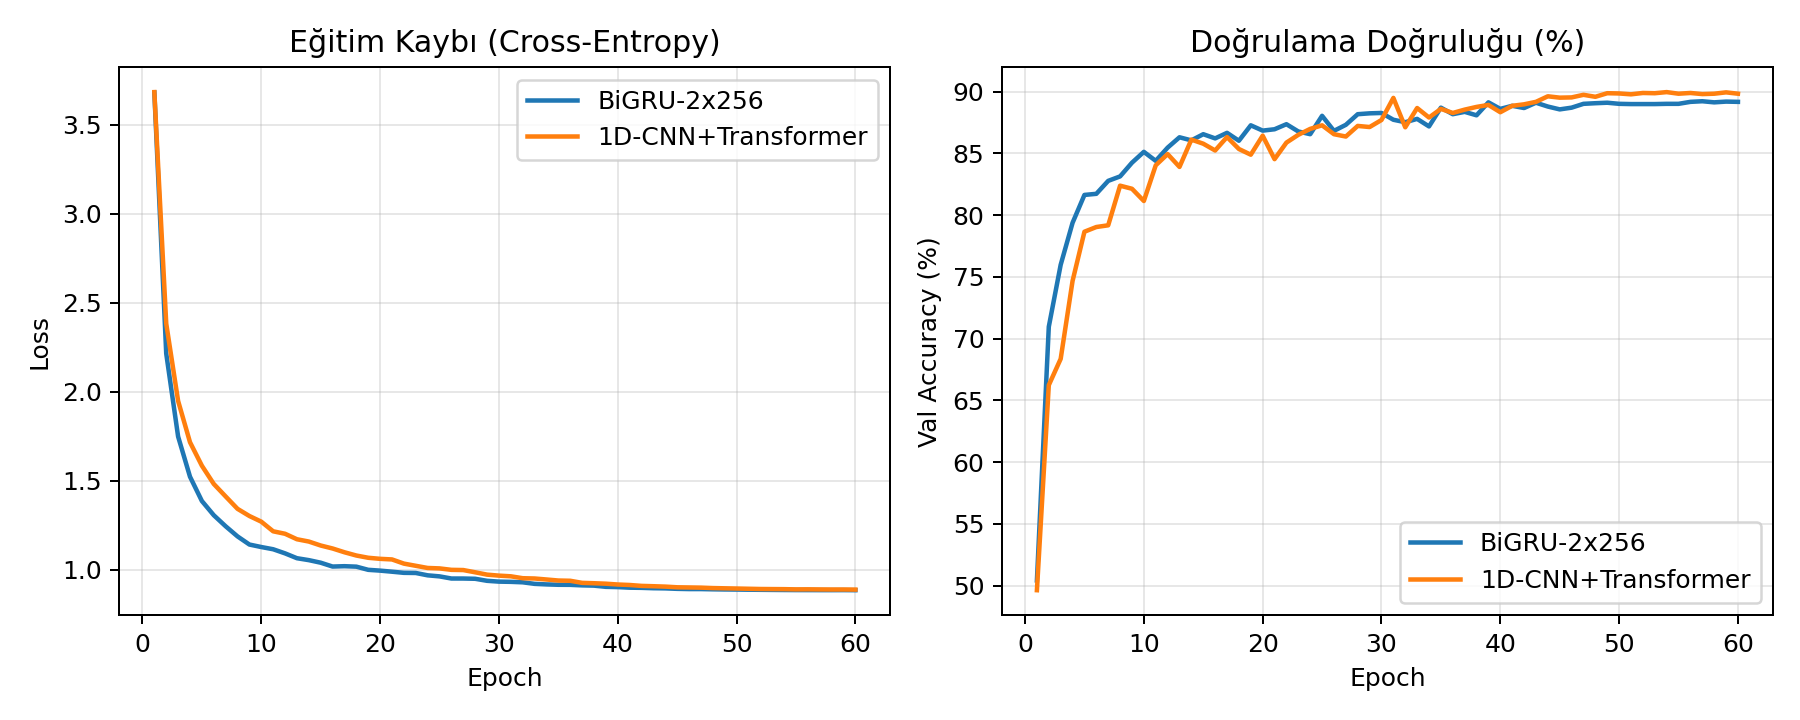
\includegraphics[width=0.95\textwidth]{grafik/egitim_egrisi.png}
\caption{BiGRU-2x256 ve 1B-CNN + Transformer modellerinin 60 epoch boyunca eğitim kaybı ve doğrulama doğruluğu eğrileri}
\label{fig:egri}
\end{figure}

Şekil~\ref{fig:egri} incelendiğinde BiGRU modelinin ilk 15 epoch'ta daha hızlı
yükseldiği, ancak 30. epoch sonrasında 1B-CNN + Transformer modelinin öne geçerek
yüzde 90,02 doğrulama ve yüzde 88,83 test doğruluğuna ulaştığı görülmektedir.
Ayrıca önceki GPU koşusunda elde edilen BiGRU ağırlıkları da yüzde 89,9 doğrulama
ve yüzde 88,0 test doğruluğu ile aynı bandı teyit etmektedir.

Hata kaynaklarını anlamak için test kümesindeki 3.741 örnek üzerinde karışıklık
matrisi ve sınıf bazlı F1 skorları çıkarılmıştır. En çok birbiriyle karışan 18
sınıfın alt karışıklık matrisi Şekil~\ref{fig:cm} üzerinde, iki modelde en sık
görülen karışma çiftleri ise Tablo~\ref{tab:karisan} içinde verilmiştir.

\begin{figure}[H]
\centering
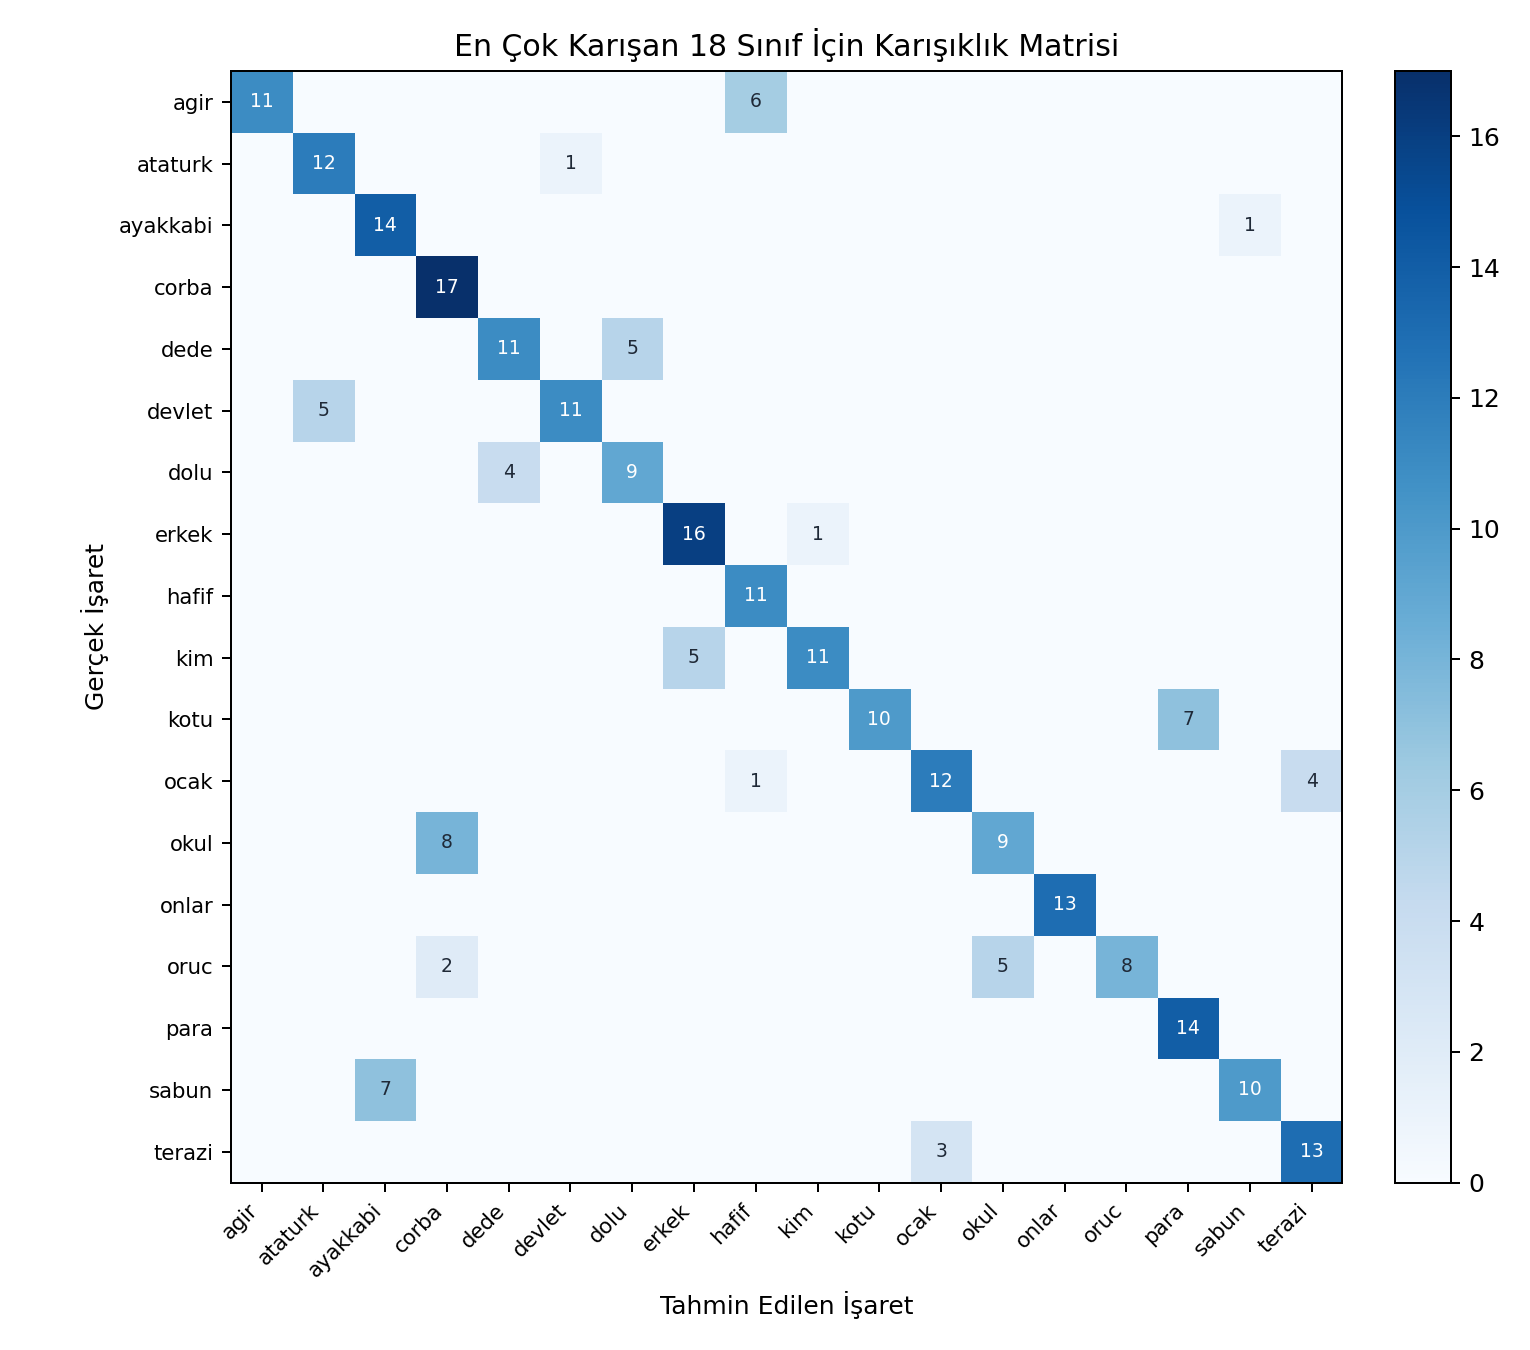
\includegraphics[width=0.88\textwidth]{grafik/karisiklik_matrisi.png}
\caption{Test kümesinde en çok karışan 18 sınıf için karışıklık matrisi (1B-CNN + Transformer)}
\label{fig:cm}
\end{figure}

\begin{table}[H]
\centering
\caption{Test kümesinde en sık birbiriyle karışan işaret çiftleri ve nedenleri}
\label{tab:karisan}
\small
\begin{tabularx}{\textwidth}{@{}l l r X@{}}
\toprule
\textbf{Gerçek İşaret} & \textbf{Tahmin Edilen} & \textbf{Hata / Toplam} & \textbf{Benzerlik Nedeni} \\
\midrule
okul (144) & çorba (43) & 8 / 17 & İki elin göğüs önünde benzer kavisli hareketi \\
kötü (122) & para (154) & 7 / 17 & Parmak ucu sürtme hareketinin 2B izdüşümde benzemesi \\
sabun (166) & ayakkabı (17) & 7 / 17 & İki elin birbirine sürtünme hareketi \\
ağır (6) & hafif (79) & 6 / 17 & Aynı iki el formu, yalnızca zıt yönlü (aşağı/yukarı) hareket \\
dede (48) & dolu (53) & 5 / 17 & Çene/ağız hizasında başlayan benzer el konumu \\
\bottomrule
\end{tabularx}
\end{table}

Tablo~\ref{tab:karisan} incelendiğinde hataların rastgele olmadığı, el formu ve
konumu aynı olup yalnızca ince parmak teması veya derinlik ekseninde ayrışan
işaretlerde toplandığı görülmektedir. Uygulamada sözlükte olmayan bir hareketin
yanlış sınıfa atanmasını engellemek için yapılan güven eşiği taramasında 0,6
eşiği seçilmiştir: bu eşiğin üzerinde kalan örnekler test kümesinin yaklaşık
yüzde 75'idir ve bu örneklerde doğruluk yüzde 96,8'e çıkmaktadır. Eşiğin altında
kalan tahminler arayüzde gösterilmemektedir.

\subsection{Mobil dönüşüm ve parite}

Eğitilen model önce NumPy ağırlıklarına aktarılmış, Keras üzerinden LiteRT
(\texttt{.tflite}) biçimine dönüştürülmüştür. Ardından dinamik aralık int8
nicemleme uygulanmıştır. Dosya boyutu fp32 sürümde 9,43 MB iken int8 sürümde
3,19 MB'a inmiştir; int8 modelin test doğruluğu yüzde 88,0 olarak aynı kalmıştır.

Dönüşümün doğru yapıldığını görmek için 200 test örneği hem Python hem telefon
üzerinde çalıştırılmış, tahminlerin yüzde 99,5'i aynı çıkmıştır. Telefonda model
çıkarımı ortalama 48 ms sürmektedir (Redmi Note 10 Pro). Ancak bu süre yalnızca
modeli kapsamaktadır. Kamera görüntüsünün alınması, MediaPipe ile el ve gövde
noktalarının çıkarılması ve arayüz güncellemesi de eklendiğinde uçtan uca hız
yaklaşık 9 FPS'e düşmektedir. Darboğaz model değil, kare başına iki ayrı MediaPipe
modelinin çalıştırılmasıdır.

Flutter arayüzü ile Kotlin tarafı arasındaki iletişim olay kanalları (event
channel) üzerinden kurulmuştur. Kamera, MediaPipe ve LiteRT işlemleri Kotlin
tarafında kalmakta, Flutter yalnızca ekranları ve durum bilgisini yönetmektedir.
